\begin{figure}[ht]
\centering
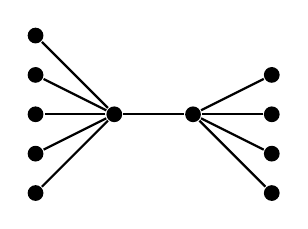
\begin{tikzpicture}[
       thick,
       acteur/.style={
         circle,
         fill=black,
         thick,
         inner sep=2pt,
         minimum size=0.2cm
       }
     ]

       \node (a1) at (0,0) [acteur]{};
       \node (a2) at (0,0.5)[acteur]{};
       \node (a3) at (0,1) [acteur]{};
       \node (a4) at (0,1.5)[acteur]{};
       \node (a5) at (0,2)[acteur]{};
       
       \node (a6) at (1,1) [acteur]{};
       \node (a7) at (2,1) [acteur]{};
       
       \node (a8) at (3,0) [acteur]{};
       \node (a9) at (3,0.5)[acteur]{};
       \node (a10) at (3,1) [acteur]{};
       \node (a11) at (3,1.5)[acteur]{};
  
       \draw (a6) -- (a7);
       
       \draw (a7) -- (a8);
       \draw (a7) -- (a9);
       \draw (a7) -- (a10);
       \draw (a7) -- (a11);
       
       \draw (a6) -- (a1);
       \draw (a6) -- (a2);
       \draw (a6) -- (a3);
       \draw (a6) -- (a4);
       \draw (a6) -- (a5);

\end{tikzpicture}
  \caption{A "weakly" connected graph}
\end{figure}
